%%%%%

\documentclass[12pt,twoside]{article}

\usepackage{weiiszablon}

\author{Karol Dudek}

% np. EF-123456, EN-654321, ...
\studentID{EF-167695}

\title{Realizacja sieci neuronowej uczonej algorytmem wstecznej propagacji błędu ucząca się rozpoznawać rodzaj schorzenia u pacjenta na podstawie wyników jego badań.}
\titleEN{Temat pracy po angielsku}


%%% wybierz rodzaj pracy wpisując jeden z poniższych numerów: ...
% 1 = inżynierska	% BSc
% 2 = magisterska	% MSc
% 3 = doktorska		% PhD
%%% na miejsce zera w linijce poniżej
\newcommand{\rodzajPracyNo}{4}


%%% promotor
\supervisor{dr hab. inż. Roman Zajdel, prof. PRz}
%% przykład: dr hab. inż. Józef Nowak, prof. PRz

%%% promotor ze stopniami naukowymi po angielsku
\supervisorEN{(academic degree) Imię i nazwisko opiekuna}

\abstract{Treść streszczenia po polsku}
\abstractEN{Treść streszczenia po angielsku}

\begin{document}

% strona tytułowa
\maketitle

\blankpage

% spis treści
\tableofcontents

\clearpage
\blankpage

\section{Wstęp}
\subsection{Cel projektu}

Głównym założeniem projektu jest realizacja sieci neuronowej uczonej za pomocą algorytmu wstecznej propagacji błędu, której zadaniem jest zdiagnozowanie zapalenia nerek lub zapalenia pęcherza na podstawie pewnych danych wejściowych.
W ramach projektu zbadano wpływ poszczególnych parametrów sieci na proces jej uczenia:
\begin{itemize}
\item S1 - ilość neuronów w I warstwy ukrytej
\item S2 - ilość neuronów w II warstwy ukrytej
\item lr (learning rate) / eta - wartość współczynnika uczenia
\item target error - maksymalny docelowy błąd sieci 
\end{itemize}
Jako zbiór danych uczących wykorzystano zbiór "Acute Inflammations”, a sama sieć została zrealizowana przy użyciu języka programowania Python.
\newpage

\subsection{Opis problemu}
Realizowana sieć na podstawie podanych informacji wejściowych ma za zadanie sklasyfikować, do której klasy należą te dane i na wyjściu podać informacje o rodzaju zdiagnowzowanej choroby.
W zbiorze danych uczących występuje 4 możliwe klasy:
\begin{itemize}
	\item brak chorób
	\item występuje zapalenie nerek
	\item występuje zapalenie pęcherza 
	\item występuje jednocześnie zapalenie pęcherza i nerek
\end{itemize}

\subsection{Opis zestawu danych}
Zestaw danych uczących został pobrany ze strony:

\textbf{https://archive.ics.uci.edu/ml/datasets/Acute+Inflammations}
 
Zbiór danych uczących zawiera 120 rekordów po 6 atrybutów w każdym wierszu.
W przypadku atrybutów, będących parametrami wejściowymi są to:
\begin{itemize}
\item a1 - Temperatura pacjenta
\item a2 - Zawroty głowy
\item a3 - Ból lędzwiowy
\item a4 - Ciągła potrzeba oddania moczu
\item a5 - Bóle mikcyjne
\item a6 - Pieczenie cewki moczowej
\end{itemize}

Oraz dwie możliwe decyzje wyjściowe:
\begin{itemize}
	\item d1 - Zapalenie pęcherza
	\item d2 - Zapalenie nerek
\end{itemize}

\subsection{Przygotowanie danych}
Badany zestaw danych nie zawiera niekompletnych rekordów, oraz wartości niepoprawnych, dlatego też podczas przygotowywania danych nie napotkano żadnych nieprzewidzianych błędów.

W celu ujednolicenia danych do poźniejszego przetwarzania na danych przeprowadzono normalizację zgodnie z poniższym wzorem:
\begin{equation}
    x_{norm}=\frac{x-x_{min}}{x_{max}-x_{min}}
    \label{Eq:normalizacja}
\end{equation}
gdzie:
\begin{itemize}
    \setlength\itemsep{0em}
    \item $x_{norm}$ - wartość po normalizacji
    \item $x$ - wartośc przed normalizacją
    \item $x_{min}$ - minimalna wartość w zbiorze
    \item $x_{max}$ – maksymalna wartość w zbiorze
\end{itemize}
Dzięki zastosowaniu wzoru~\ref{Eq:normalizacja} pierwotne dane wejściowe każdego rekordu zostały zamienione na odpowiadające im wartości z zakresu od 0 do 1.

\clearpage

\section{Zagadnienia teorytyczne}
\subsection{Model sztucznego neuronu}
Każda sieć neuronowa składa się z połączonych między sobą pojedynczych neuronów. Należy zatem zapoznać się z modelem pojedynczego neuronu w celu zrozumienia problemu sieci neuronowych. Przykładowy model pojedynczego neuronu został przedstawiony na rysunku~\ref{Fig:neuron}
\begin{figure}[ht!]
	\centering
	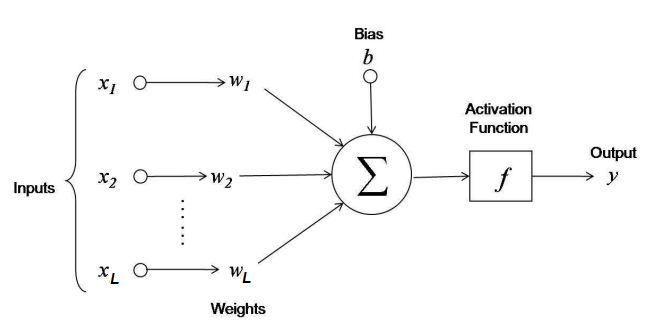
\includegraphics[width=12cm]{figures/model_neuronu.png}
	\caption{Model pojedynczego neuronu}
	\label{Fig:neuron}
\end{figure}

Każdy neuron to układ składający się z wielu wejść i jednego wyjścia. Wszystkie wejścia posiadają tzw. współczynnik wagowy, który określa jak bardzo dane wejście wpływa na rezultat wynikowy danego neuronu. Oprócz wagi dodatkowym elementem wejściowych jest również bias, umożliwiający przesunięcie funkcji aktywacji w lewo lub w prawo danego neuronu.
Całość z poprzednio podanych informacji do wejść neuronu trafia do sumatora gdzie odbywa się proces wyznaczania łącznego pobudzenia
neuronu, wyrażanego z następującego wzoru~\ref{Eq:pobudzenie}:
\begin{equation}
	z = \sum_{j=1}^{L} w_{j}x_{j}+b
	\label{Eq:pobudzenie}
\end{equation}
Wyznaczona wartość następnie trafia do funkcji aktywacji, gdzie określany jest sygnał wyjściowy neuronu zgodnie z zależnością \ref{Eq:aktywacja}:
\newpage
\begin{equation}
	y = f(z) = f(\sum_{j=1}^{L} w_{j}x_{j}+b)
	\label{Eq:aktywacja}
\end{equation}
gdzie:
\begin{itemize}
	\item $y$ - wyjście neuronu
	\item $x_{j}$ - \textit{j}-ty sygnał wejściowy (\textit{j=1,2,\dots,L})
	\item $w_{j}$ - waga \textit{j}-tego wejścia
	\item $b$ - bias
\end{itemize}
\subsection{Funkcja aktywacji}
Każda warstwa w swoich neuronach może wykorzystywać inną funkcję aktywacji.
W przypadku sieci jednokierunkowych najbardziej powszechna jest funkcja sigmoidalna, w której wyróżnić można dwa typy:
\begin{itemize}
	\item unipolarna funkcja aktywacji, która przyjmuje wartości w przedziału (0,1):
\end{itemize}
\begin{equation}
	f(x) = \frac{1}{1+e^{-x}}
	\label{Eq:unipolar_sigmoid}
\end{equation}
\begin{itemize}[resume]
	\item bipolarna funkcja aktywacji, przyjmująca wartości z przedziału (-1,1):
\end{itemize}
\begin{equation}
	f(x) = \frac{2}{1+e^{-x}} - 1
	\label{Eq:bipolar_sigmoid}
\end{equation}
Funkcje te są różniczkowalne i ich pochodne wyrazić można jako:
\begin{itemize}
	\item w przypadku unipolarnej funkcji aktywacji:
\end{itemize}
\begin{equation}
	f(x) = \frac{1}{1+e^{-x}}(1-\frac{1}{1+e^{-x}})
	\label{Eq:unipolar_sigmoid_pochodna}
\end{equation}
\begin{itemize}[resume]
	\item w przypadku bipolarnej funkcji aktywacji:
\end{itemize}
\begin{equation}
	f(x) = 1 - (\frac{2}{1+e^{-x}})^2
	\label{Eq:bipolar_sigmoid_pochodna}
\end{equation}
\newpage
\subsection{Model sieci wielowarstwowej}
W każdej sieci jednokierunkowej wielowarstwowej wyróżnić można nastepujące warstwy: wejścia, wyścia i występujące pomiędzy nimi warstwy ukryte.
W przypadku sieci jednokierunkowej dane mogą przepływać tylko w jednym kierunku od warstwy wejścia do warstwy wyjścia.
\begin{figure}[ht!]
	\centering
	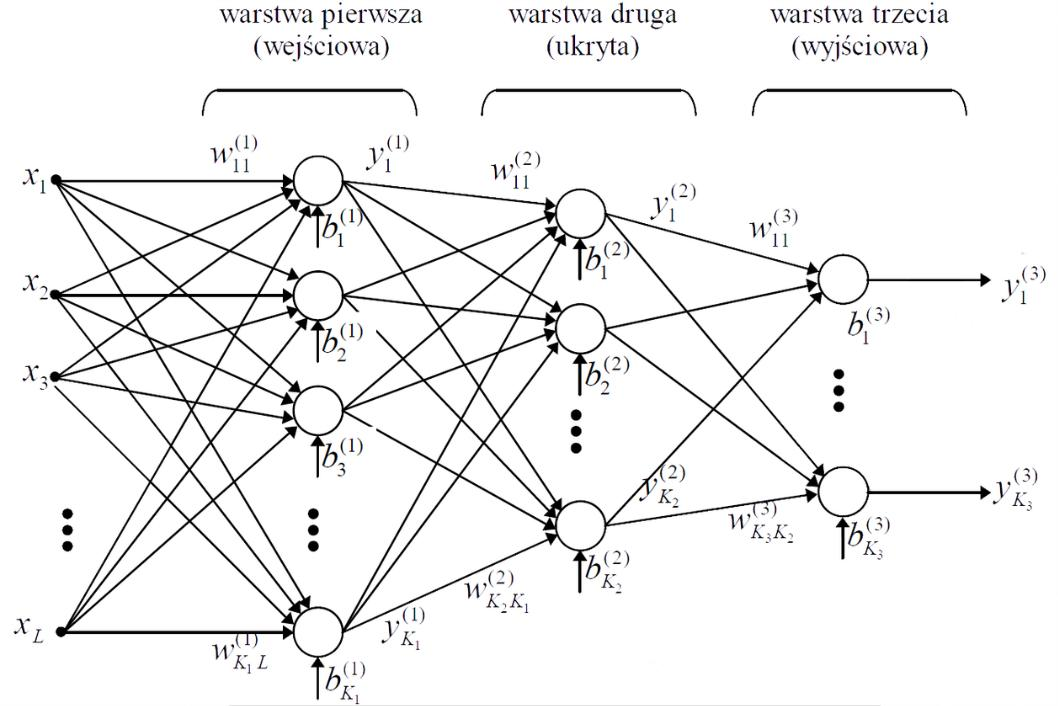
\includegraphics[width=12cm]{figures/model_sieci.png}
	\caption{Model sieci jednokierunkowej wielowarstwowej}
	\label{Fig:model_sieci}
\end{figure}

Każda pojedyncza warstwa neuronów posiada:
\begin{itemize}
	\item macierz wag \textbf{w}
\end{itemize}
\begin{itemize}[resume]
	\item wektor przesunieć \textbf{b}
\end{itemize}
\begin{itemize}[resume]
	\item funkcje aktywacji \textbf{f}
	\item oraz wektor sygnałów wyjściowych \textbf{y}
\end{itemize}
W celu obliczenia sygnału wyjściowego sieci wielowarstwowej uogólniony wzór na wyjście pojedynczej warstwy przedstawiający się jako:
\begin{equation}
	y^{(n)}=f^{(n)}(w^{(n)}y^{(n-1)}+b^{(n)})
\end{equation}
gdzie $n$ to numer odpowiedniej warstwy.

Dla przykładu dla przedstawionej sieci~\ref{Fig:model_sieci} wzory opisujące wyjścia poszczególnych warstw przyjmą postać:
\begin{equation}
	y^{(1)} = f^{(1)}(w^{(1)}x+b^{(1)})
\end{equation}
\begin{equation}
	y^{(2)} = f^{(2)}(w^{(2)}y^{(1)}+b^{(2)})
\end{equation}
\begin{equation}
	y^{(3)} = f^{(3)}(w^{(3)}y^{(2)}+b^{(3)})
\end{equation}
Na podstawie powyższych równań sygnał wyjściowy całej sieci~\ref{Fig:model_sieci} można opisać wzorem:
\begin{equation}
	y^{(3)}=f^{(3)}(w^{(3)}f^{(2)}(w^{(2)}f^{(1)}(w^{(1)}x+b^{(1)})+b^{(2)})+b^{(3)})
	\label{Eq:y_sieci}
\end{equation}
\newpage
\subsection{Uczenie sieci pod nadzorem (supervised learning)}
Uczenie z nadzorem polega na wprowadzaniu do systemu uczącego się próbki danych (danych uczących) posiadającej pary danych w postaci tzw. wektora wejściowego i wektora wyjściowego, gdzie:
\begin{itemize}
	\setlength\itemsep{0em}
	\setlength{\parskip}{0pt}
	\item wektor wejściowy - wektor podawany na wejście sieci
	\item wektor wyjściowy - wektor oczekiwanych wartości na wyjściu sieci
\end{itemize}
Zatem ten sposób uczenia zakłada, że każdemu wektorowi wejściowemu towarzyszy wektor wyjściowy. Taka para jest wykorzystywana w procesie uczenia, a dokładnie zmiany wag i biasów neuronów w kolejnych jego cyklach.
W sieci nienauczonej w większości przypadków sygnał wyjściowy $y$ będzie inny niż oczekiwany $\hat{y}$. Taki błąd nazywa się funkcją straty, która według wzoru dla pojedynczego neuronu wyjściowego przedstawić można jako:
\begin{equation}
	e_{i}=y_{i}-\hat{y_{i}}
\end{equation}
Funkcja straty w poźniejszej fazie wykorzystywana jest do obliczenia wartości tzw. funkcji kosztu, która w bezpośredni sposób bierze udział w procesie uczenia. Najczęsciej stosowaną funkcją kosztu dla klasyfikacji to:
\begin{itemize}
	\item SSE (Sum Squared Error) - sumaryczny błąd kwadratowy:
\end{itemize}
\begin{equation}
	E = \frac{1}{2} \sum_{i=1}^{K} e_{i}^{2}
\end{equation}
gdzie:
\begin{itemize}
	\setlength\itemsep{0em}
	\setlength{\parskip}{0pt}
	\item $i$ - numer neuronu w warstwie wyjściowej
	\item $K$ - ilość neuronów w warstwie wyjściowej.
\end{itemize}
Korzystając z wzoru opisującego sygnał wyjściowy sieci~\ref{Eq:y_sieci} można przedstawić pełne rozwinięcie funkcji celu:
\begin{equation}
	\begin{aligned}
		E &= \frac{1}{2} \sum_{i_3=1}^{K_3}e_{i_3}^2
		= \frac{1}{2} \sum_{i_3=1}^{K_3}(y_{i_3}^{(3)} - \hat{y_{i_3}})^2\\
		&= \frac{1}{2} \sum_{i_3=1}^{K_3}(f^{(3)}(w^{(3)}f^{(2)}(w^{(2)}f^{(1)}(w^{(1)}x+b^{(1)})+b^{(2)})+b^{(3)}) - \hat{y_{i_3}})^2\\
		&= \frac{1}{2}\sum_{i_3=1}^{K_3}(f^{(3)}(\sum_{i_2=1}^{K_2}w_{i_3i_2}^{(3)}y_{i_2}+b_{i_3}^{(3)}) - \hat{y_{i_3}})^2\\
		&= \frac{1}{2}\sum_{i_3=1}^{K_3}(
		f^{(3)}(\sum_{i_2=1}^{K_2}w_{i_3i_2}^{(3)}f^{(2)}(
		\sum_{i_1=1}^{K_1}w_{i_2i_1}^{(2)}y_{i_1}+b_{i_2}^{(2)}
		)+b_{i_3}^{(3)}) - \hat{y_{i_3}})^2\\
		&= \frac{1}{2}\sum_{i_3=1}^{K_3}(
		f^{(3)}(\sum_{i_2=1}^{K_2}w_{i_3i_2}^{(3)}f^{(2)}(
		\sum_{i_1=1}^{K_1}w_{i_2i_1}^{(2)}
		f^{(1)}(\sum_{j=1}^{L}w_{i_1j}^{(1)}x_j+b_{i_1}^{(1)})
		+b_{i_2}^{(2)}
		)+b_{i_3}^{(3)})
		- \hat{y_{i_3}})^2
	\end{aligned}
	\label{Eq:funkcja_celu}
\end{equation}
gdzie:
\begin{itemize}
	\setlength\itemsep{0em}
	\setlength{\parskip}{0pt}
	\item $j = 1,\dots,L$ numer wejścia warstwy I
	\item $j_1=1,\dots,K_1$, $j_1=1,\dots,K_1$, $j_1=1,\dots,K_1$ odpowiednio numer wyjścia warstwy~I,~II,~III
\end{itemize}
\newpage

\subsection{Algorytm wstecznej propagacji błędu}
Podczas uczenia sieci neuronowych celem każdego zastosowanego algorytmu jest modyfikowanie wag danego neuronu w taki sposób, aby na wyjściu sieć popełniała jak najmniejszy błąd. Obecnie najbardziej rozpowszechnione są dwa rodzaje / sposoby uczenia sieci. Pierwszy sposób polega na aktulizacji wag po przejściu wszystkich danych uczących. Drugi natomiast za pomocą gradientów i reguły łańcuchowej
powracaniu do początku sieci i rozkładaniu odpowiednio wartości błędów próbując poprawić wagi. Proces ten nazwę propagacji wstecznej.

Na początku jedyną rzeczą jaką można wyznaczyć to błędy neuronów warstwy wyjściowej na podstawie danych wyjściowych i danych docelowych zawartych w zbiorze uczącym. Kolejne błędy w warstwach wcześniejszych niż wyjściowa będą określane dzięki algorytmowi wstecznej propagacji.
Wzór umożliwiający obliczenie zmiany wagi przedstawia się jako:
\begin{equation}
	\Delta w_{ij} = - \eta\frac{\partial E}{\partial w_{ij}}
	\label{Eq:delta_wagi}
\end{equation}
gdzie $\eta$ oznacza wartość współczynnika uczenia
Opisując algorytm można dojść do wniosku, że należy on do metod gradientowych, gdyż jego założenie opiera sie na stwierdzeniu, że gradient funkcji wskazuje na kierunek jej najszybszego wzrostu, a przy zmianie znaku na przeciwny kierunek jej najszybszego spadku.
Zakładając, że każda zmiana wagi zależy od danej chwili uczenia $t$ (tutaj zwykle epoki) wartość danej wagi można zapisać jako:
\begin{equation}
	w_{ij}(t+1) = w_{ij}(t)+\Delta w_{ij}
\end{equation}
Podstawienie równania~\ref{Eq:delta_wagi} pozwala na przekształcenie powyższego wzoru do postaci:
\begin{equation}
	w_{ij}(t+1) = w_{ij}(t) - \eta\frac{\partial E}{\partial w_{ij}}
\end{equation}
Przy obliczaniu gradientu dla danej wagi, napotyka się problem o niemożności określenia go za pomocą bezpośrednich obliczeń, dlatego też najpierw należy określić wygląd poszczególnych pochodnych cząstkowych z zależności~\ref{Eq:funkcja_celu}, a następnie na ich podstawie odpowiadający danej wadze gradient:
\begin{itemize}
	\item dla warstwy wyjściowej:
\end{itemize}
\begin{equation}
	\frac{\partial E}{\partial w_{i_3i_2}^{(3)}}= \frac{\partial E}{\partial f^{(3)}}\frac{\partial f^{(3)}(z_{i_3}^{(3)})}{\partial z_{i_3}^{(3)}}\frac{\partial z_{i_3}^{(3)}}{\partial w_{i_3i_2}^{(3)}} = (y_{i_3} - \hat{y_{i_3}}) \frac{\partial f^{(3)}(z_{i_3}^{(3)})}{\partial z_{i_3}^{(3)}}y_{i_2}^{(2)}
\end{equation}
gdzie: $z_{i_3}^{(3)} = \sum_{i_2=1}^{K_2} w_{i_3i_2}^{(3)}y_{i_2}+b_{i_3}^{(3)}$ - pobudzenie $i_3$-ego neuronu warstwy wyjściowej.

\begin{itemize}[resume]
	\item dla warstwy ukrytej:
\end{itemize}
\begin{equation}
	\begin{aligned}
		\frac{\partial E}{\partial w_{i_2i_1}^{(3)}}&= \frac{\partial E}{\partial f^{(3)}}\frac{\partial f^{(3)}(z_{i_3}^{(3)})}{\partial z_{i_3}^{(3)}}\frac{\partial z_{i_3}^{(3)}}{\partial f^{(2)}} \frac{\partial f^{(2)}(z_{i_2}^{(2)})}{\partial z_{i_2}^{(2)}}\frac{\partial z_{i_2}^{(2)}}{\partial w_{i_2i_1}^{(2)}}\\
		&= \sum_{i_3=1}^{K_3} (y_{i_3} - \hat{y_{i_3}}) \frac{\partial f^{(3)}(z_{i_3}^{(3)})}{\partial z_{i_3}^{(3)}} w_{i_3i_2}^{(3)}
		\frac{\partial f^{(2)}(z_{i_2}^{(2)})}{\partial z_{i_2}^{(2)}} y_{i_1}^{(1)}
	\end{aligned}
\end{equation}

\begin{itemize}[resume]
	\item dla warstwy wejściowej:
\end{itemize}
\begin{equation}
	\begin{aligned}
		\frac{\partial E}{\partial w_{i_1j}^{(3)}}&= \frac{\partial E}{\partial f^{(3)}}\frac{\partial f^{(3)}(z_{i_3}^{(3)})}{\partial z_{i_3}^{(3)}}\frac{\partial z_{i_3}^{(3)}}{\partial f^{(2)}} \frac{\partial f^{(2)}(z_{i_2}^{(2)})}{\partial z_{i_2}^{(2)}}\frac{\partial z_{i_2}^{(2)}}{\partial f^{(1)}}
		\frac{\partial f^{(1)}(z_{i_1}^{(1)})}{\partial z_{i_1}^{(1)}}\frac{\partial z_{i_1}^{(1)}}{\partial w_{i_1j}^{(1)}}\\
		&= \sum_{i_3=1}^{K_3} (y_{i_3} - \hat{y_{i_3}}) \frac{\partial f^{(3)}(z_{i_3}^{(3)})}{\partial z_{i_3}^{(3)}} \sum_{i_2=1}^{K_2} w_{i_3i_2}^{(3)}
		\frac{\partial f^{(2)}(z_{i_2}^{(2)})}{\partial z_{i_2}^{(2)}} w_{i_2i_1}^{(2)} \frac{\partial f^{(1)}(z_{i_1}^{(1)})}{\partial z_{i_1}^{(1)}} x_j
	\end{aligned}
\end{equation}
\newpage

\clearpage

\section{Realizacja sieci}

\subsection{Opis skryptu}

Na potrzeby realizacji sieci neuronowej stworzono skrypt w języku Python umożliwiającą w prosty sposób zrealizować dowolną sieć neuronową uczoną metodą wstecz nej propagracji błędu.
Skrypt został podzielony na 3 pliki: network.py, data.py oraz main.py.
Skrypt data.py miał za zadanie prygotować dane pobrane ze zbioru danych do optymalnego formatu dla sieci neuronowej. Skrypt network.py zawierał cały kod sieci neuronowej, natomiast skrypt main.py łączył 2 wcześniej wspomniane skrypty.

\begin{lstlisting}[caption={Plik przygotowujący dane- data.py},label={Lst:data_py},language=Python,basicstyle=\scriptsize]
from sklearn.model_selection import train_test_split
from csv import reader
import numpy as np

# Import function
def dataImport(name):
    with open(name, 'r', encoding='utf-16') as file:
        return [line for line in reader(file, delimiter='\t')]

# Normalization function
def normalizeMinMax(table):
    for row in range(0, len(table)):
        min_val, max_val = min(table[row]), max(table[row])
        table[row] = [(1 - 0) * (col - min_val) / (max_val - min_val) for col in table[row]]
    return table

# Data loader function
def loadData():
    # Import acute.tsv to dataFile
    dataFile = dataImport('acute.tsv')

    # Create numpy array from dataList
    dataFile = np.array(dataFile)

    # Convert array of strings to array of floats
    dataFile = dataFile.astype(float)

    # Data normalization
    dataFile = normalizeMinMax(dataFile.T).T

    # Data splitting into training and test data
    trainData, testData = train_test_split(dataFile, test_size=0.2, random_state=25)

    # Splitting data into 2 groups, inputData and outputdata
    testIn, testOut = testData[:,:6], testData[:,6:]
    trainIn, trainOut = trainData[:,:6], trainData[:,6:]

    # Combining inputData and outputData in a single tuple
    trainData = [(np.array(trainIn[i], ndmin=2).T, np.array(trainOut[i], ndmin=2).T) for i in range(0, len(trainOut))]
    testData = [(np.array(testIn[i], ndmin=2).T,np.array(testOut[i], ndmin=2).T) for i in range(0, len(testOut))]

    return (trainData, testData)
\end{lstlisting}

\begin{lstlisting}[caption={Plik zawierający sieć - network.py},label={Lst:network_py},language=Python,basicstyle=\scriptsize]
import random
import time
import numpy as np

class Network(object):

    # Constructor, takes list of layers and amount of neurons as parameter
    def __init__(self, sizes):

        #Applying Seed
        np.random.seed(7)

        # Assing 'sizes' vector to amount of layers in the network
        self.num_layers = len(sizes)
        self.sizes = sizes

        # Pseudo random generator used to assign weight and biases 
        self.biases = [np.random.randn(y, 1) for y in sizes[1:]]
        self.weights = [np.random.randn(y, x)
                        for x, y in zip(sizes[:-1], sizes[1:])]

    def feedforward(self, a):

        # Return neural network results for 'a' data
        for b, w in zip(self.biases, self.weights):
            a = sigmoid(np.dot(w, a)+b)
        return a

        # Mean Square Error
    def mse(self,_test_data):
        error=[pow(np.linalg.norm(self.feedforward(x)-y),2) for (x,y) in _test_data]
        return 1/len(_test_data)*sum(error)

    def SGD(self, training_data, epochs, mini_batch_size, eta,
            error_target=0.001, test_data=None):

        if test_data: n_test = len(test_data)
        n = len(training_data)
        for j in range(epochs):
            time1 = time.time()
            random.shuffle(training_data)
            mini_batches = [
                training_data[k:k+mini_batch_size]
                for k in range(0, n, mini_batch_size)]
            for mini_batch in mini_batches:
                self.update_mini_batch(mini_batch, eta)
            cur_err = self.mse(training_data)
            time2 = time.time()
            evalVal = self.evaluate(test_data)
            evalAcc = (evalVal/n_test*100)
            if cur_err < error_target or j == epochs-1:
                if test_data:
                    print("{0}, {2:.2f}, {3:.0f}%".format(
                        j, cur_err, evalAcc))
                    pass
                else:
                    print("Epoch {0} ".format(j))
                break

            print("{0}, {1:.6f}, {2:.0f}%".format(j, cur_err, evalAcc))

    def update_mini_batch(self, mini_batch, eta):

        # Updates weights and biases using SGD and backpropagation for each mini batch
        nabla_b = [np.zeros(b.shape) for b in self.biases]
        nabla_w = [np.zeros(w.shape) for w in self.weights]
        for x, y in mini_batch:
            # Calculate gradient increase for each (x, y) pair
            delta_nabla_b, delta_nabla_w = self.backprop(x, y)

            # Calculate new gradient
            nabla_b = [nb+dnb for nb, dnb in zip(nabla_b, delta_nabla_b)]
            nabla_w = [nw+dnw for nw, dnw in zip(nabla_w, delta_nabla_w)]

        # New weights and biases
        self.weights = [w-(eta/len(mini_batch))*nw
                        for w, nw in zip(self.weights, nabla_w)]
        self.biases = [b-(eta/len(mini_batch))*nb
                       for b, nb in zip(self.biases, nabla_b)]

    def backprop(self, x, y):

        #Return tuple representing the gradient of the cost function
        nabla_b = [np.zeros(b.shape) for b in self.biases]
        nabla_w = [np.zeros(w.shape) for w in self.weights]

        # feedforward
        activation = x
        activations = [x] # list to store all the activations, layer by layer
        zs = [] # list to store all the z vectors, layer by layer
        
        # Calculate neuron activations
        for b, w in zip(self.biases, self.weights):
            z = np.dot(w, activation)+b
            zs.append(z)
            activation = sigmoid(z)
            activations.append(activation)

        # backward pass (gradient increase for output layer)
        delta = self.cost_derivative(activations[-1], y) * \
            sigmoid_prime(zs[-1])
        nabla_b[-1] = delta
        nabla_w[-1] = np.dot(delta, activations[-2].transpose())

        # Calculate gradient increase for input and hidden layers
        for l in range(2, self.num_layers):
            z = zs[-l]
            sp = sigmoid_prime(z)
            delta = np.dot(self.weights[-l+1].transpose(), delta) * sp
            nabla_b[-l] = delta
            nabla_w[-l] = np.dot(delta, activations[-l-1].transpose())
        return (nabla_b, nabla_w)

    def evaluate(self, test_data):

        test_results = [(self.feedforward(x), y)
                        for (x, y) in test_data]

                        # Approximation
        return sum(int((y[0] == 0 and x[0] < 0.5) or (y[0] == 1 and x[0] > 0.5) and 
                       (y[1] == 0 and x[1] < 0.5) or (y[1] == 1 and x[1] > 0.5)) 
                   for (x, y) in test_results)

    def cost_derivative(self, output_activations, y):
        # Return vector with difference between the neuron and the expected result
        return (output_activations-y)

#### Miscellaneous functions
def sigmoid(z):
    # Sigmoid function
    return 1.0/(1.0+np.exp(-z))

def sigmoid_prime(z):
    # Sigmoid prime function
    return sigmoid(z)*(1-sigmoid(z))


\end{lstlisting}

\begin{lstlisting}[caption={Plik wywołujący przykładową sieć - main.py},label={Lst:main_py},language=Python,basicstyle=\scriptsize]
	import data
	import network
	
	import numpy as np
	
	trainData, testData = data.loadData()
	
	# [input vector size, S1 neurons, S2 neurons, output]
	net = network.Network([6,2])
	
	# (training_data, epochs, batch_size, eta, target, test_data)
	net.SGD(trainData, 100000, 1, 0.1, error_target=0.179,test_data=testData)
\end{lstlisting}

\clearpage	

\section{Eksperymenty}
\subsection{Eksperyment 1}
Celem pierwszego eksperymentu było sprawdzenie jak wielkość partii danych uczących wpływa na szybkość uczenia się sieci.
W tym eksperymencie parametry sieci jednowarstwowej były następujące:
\begin{itemize}
	\item epoki - 10000
	\item learning rate - 0,3
	\item target error - 0,179
\end{itemize}

\begin{figure}[ht!]
	\centering
	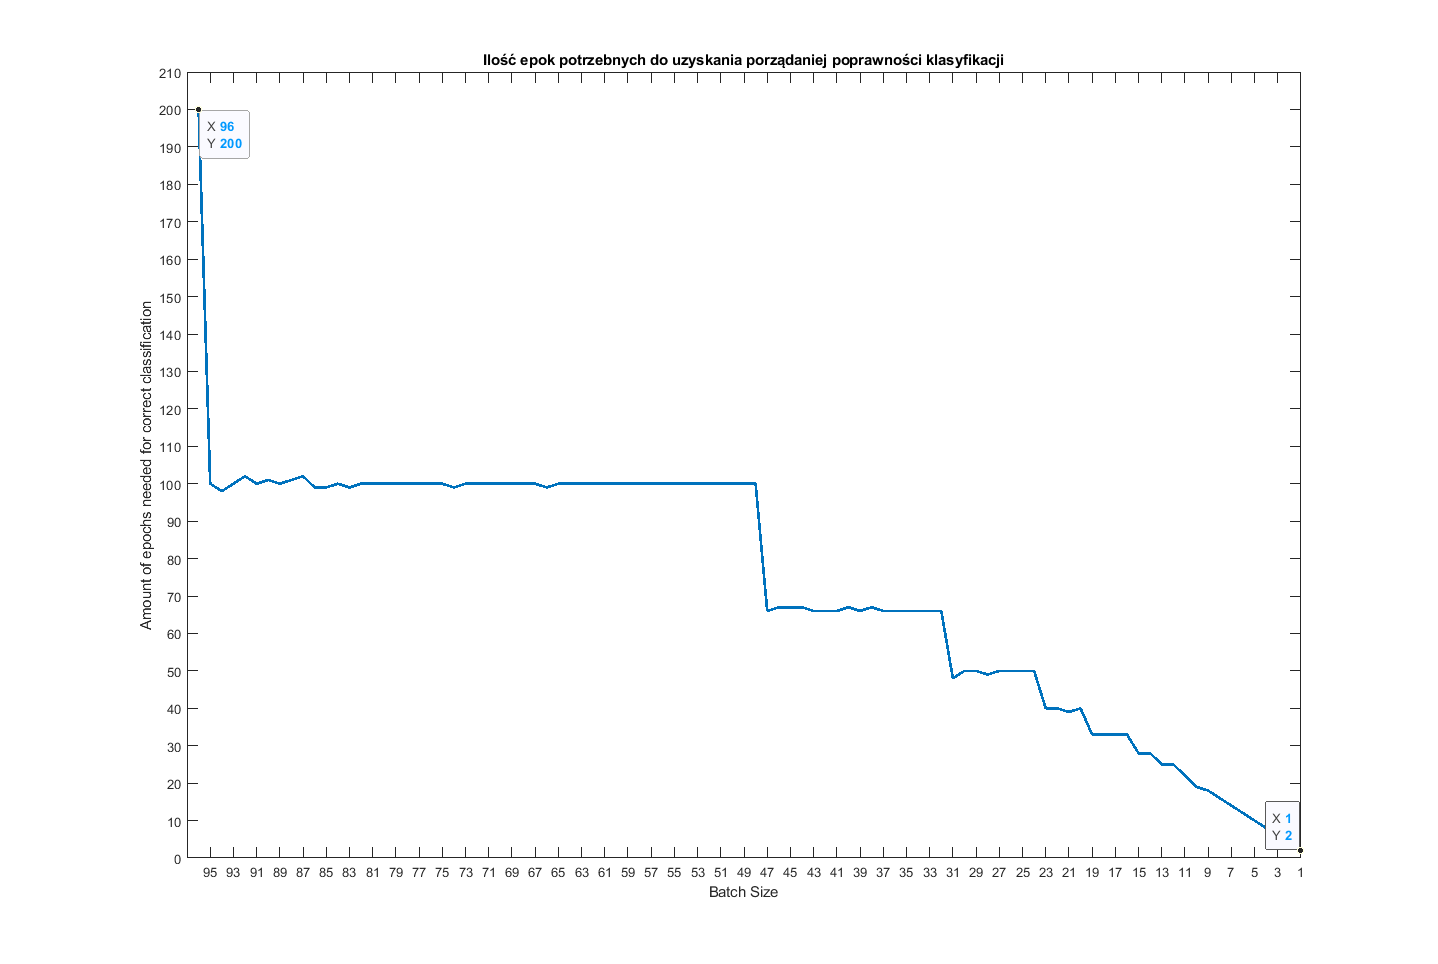
\includegraphics[width=15cm]{figures/batch_epo.png}
	\caption{Wykres do eksperymentu pierwszego}
\end{figure}
Z powyższego wykresu możemy zauważyć, iż batch size wielkości 1 wypada najlepiej pod kątem szybkości uczenia się sieci.
\newpage



\subsection{Eksperyment 2}
Celem drugiego eksperymentu było sprawdzenie jak learning rate wpływa na szybkość uczenia się sieci.
W tym eksperymencie parametry sieci jednowarstwowej były następujące:
\begin{itemize}
	\item epoki - 10000
	\item batch size - 1
	\item target error - 0,18
\end{itemize}

\begin{figure}[ht!]
	\centering
	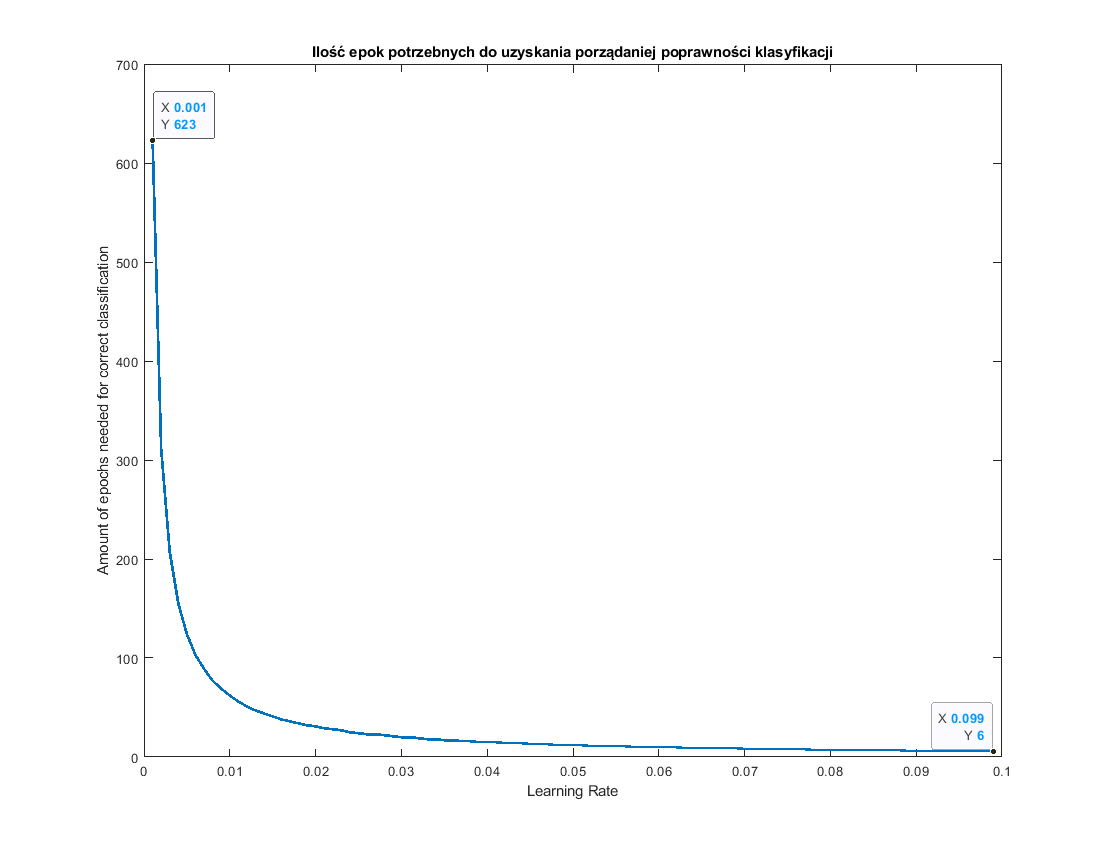
\includegraphics[width=15cm]{figures/eta_epo.png}
	\caption{Wykres do eksperymentu drugiego}
\end{figure}
Z wykresu można zauważyć jak ilość epok potrzebnych do osiągniecia porządanej klasyfikacji spada wraz ze wzrostem learning rate.
\newpage

\subsection{Eksperyment 3}
Celem trzeciego eksperymentu było sprawdzenie jak błąd docelowy wpływa na szybkość uczenia się sieci.
W tym eksperymencie parametry sieci jednowarstwowej były następujące:
\begin{itemize}
	\item epoki - 10000
	\item learning rate - 0,01
	\item batch size - 1
\end{itemize}

\begin{figure}[ht!]
	\centering
	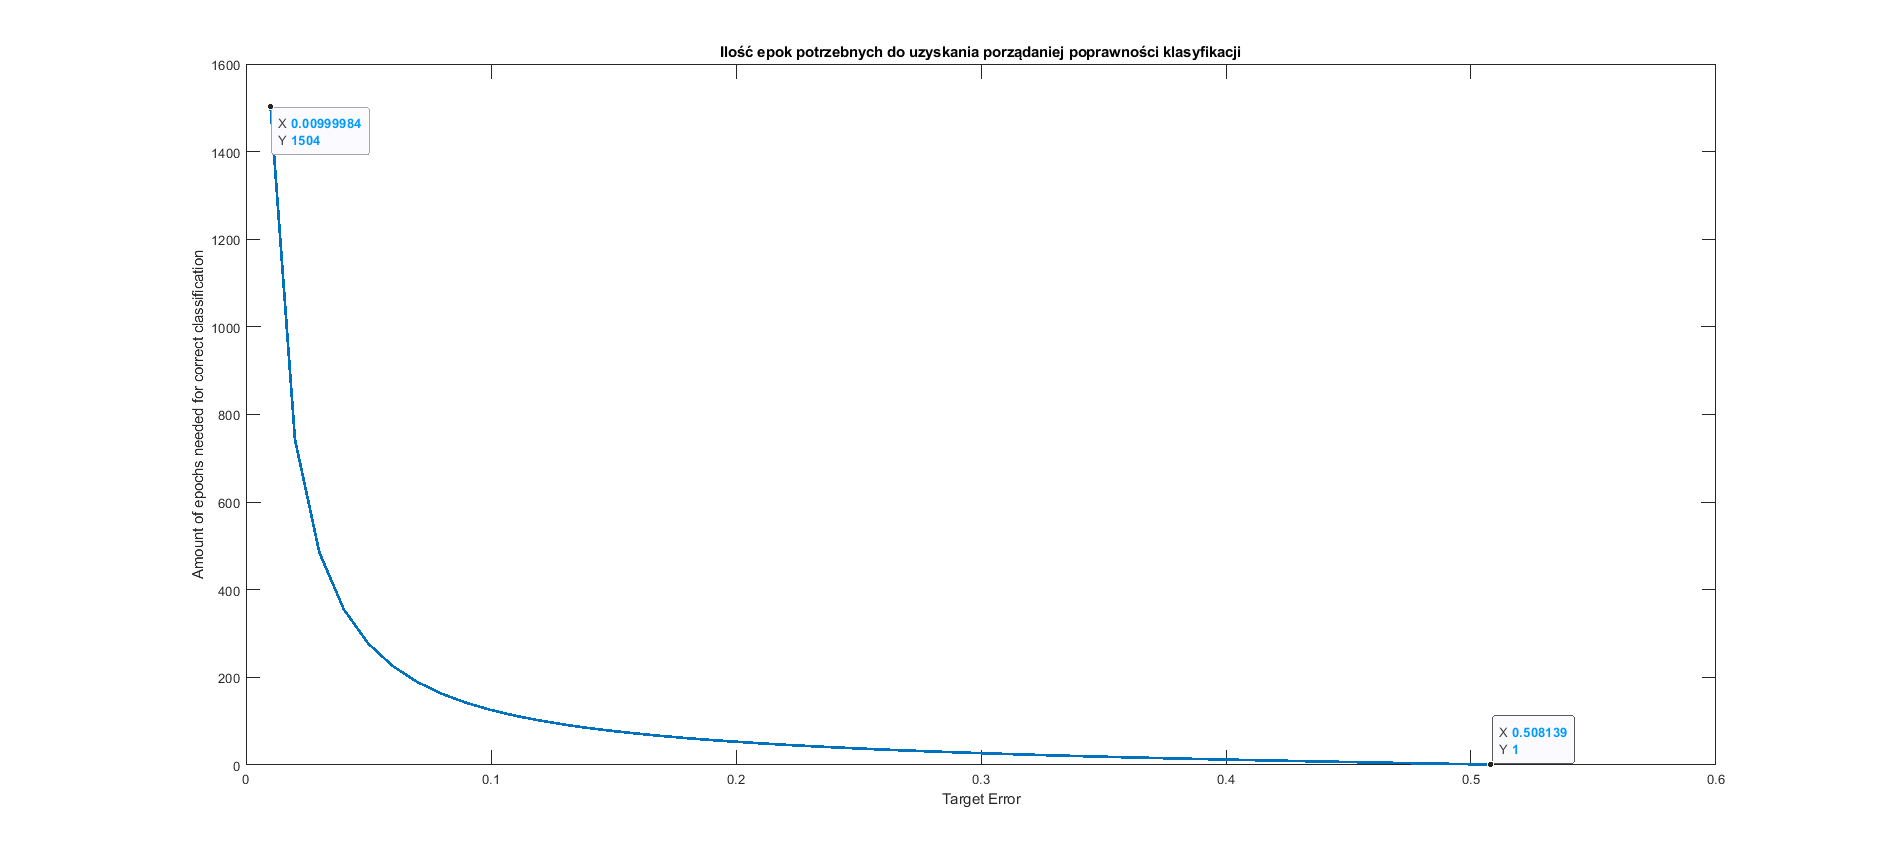
\includegraphics[width=15cm]{figures/target_epo_eta=0_01.png}
	\caption{Wykres do eksperymentu trzeciego}
\end{figure}
Na wykresie możemy zauważyć spadek epok potrzebnych do osiągniecia porządanej klasyfikacji wraz ze wzrostem błędu docelowego.
\newpage

\subsection{Eksperyment 4}
Celem czwartego eksperymentu było sprawdzenie jak błąd docelowy wpływa na szybkość uczenia się sieci.
W tym eksperymencie parametry sieci jednowarstwowej były następujące:
\begin{itemize}
	\item epoki - 10000
	\item learning rate - 0,1
	\item batch size - 1
\end{itemize}

\begin{figure}[ht!]
	\centering
	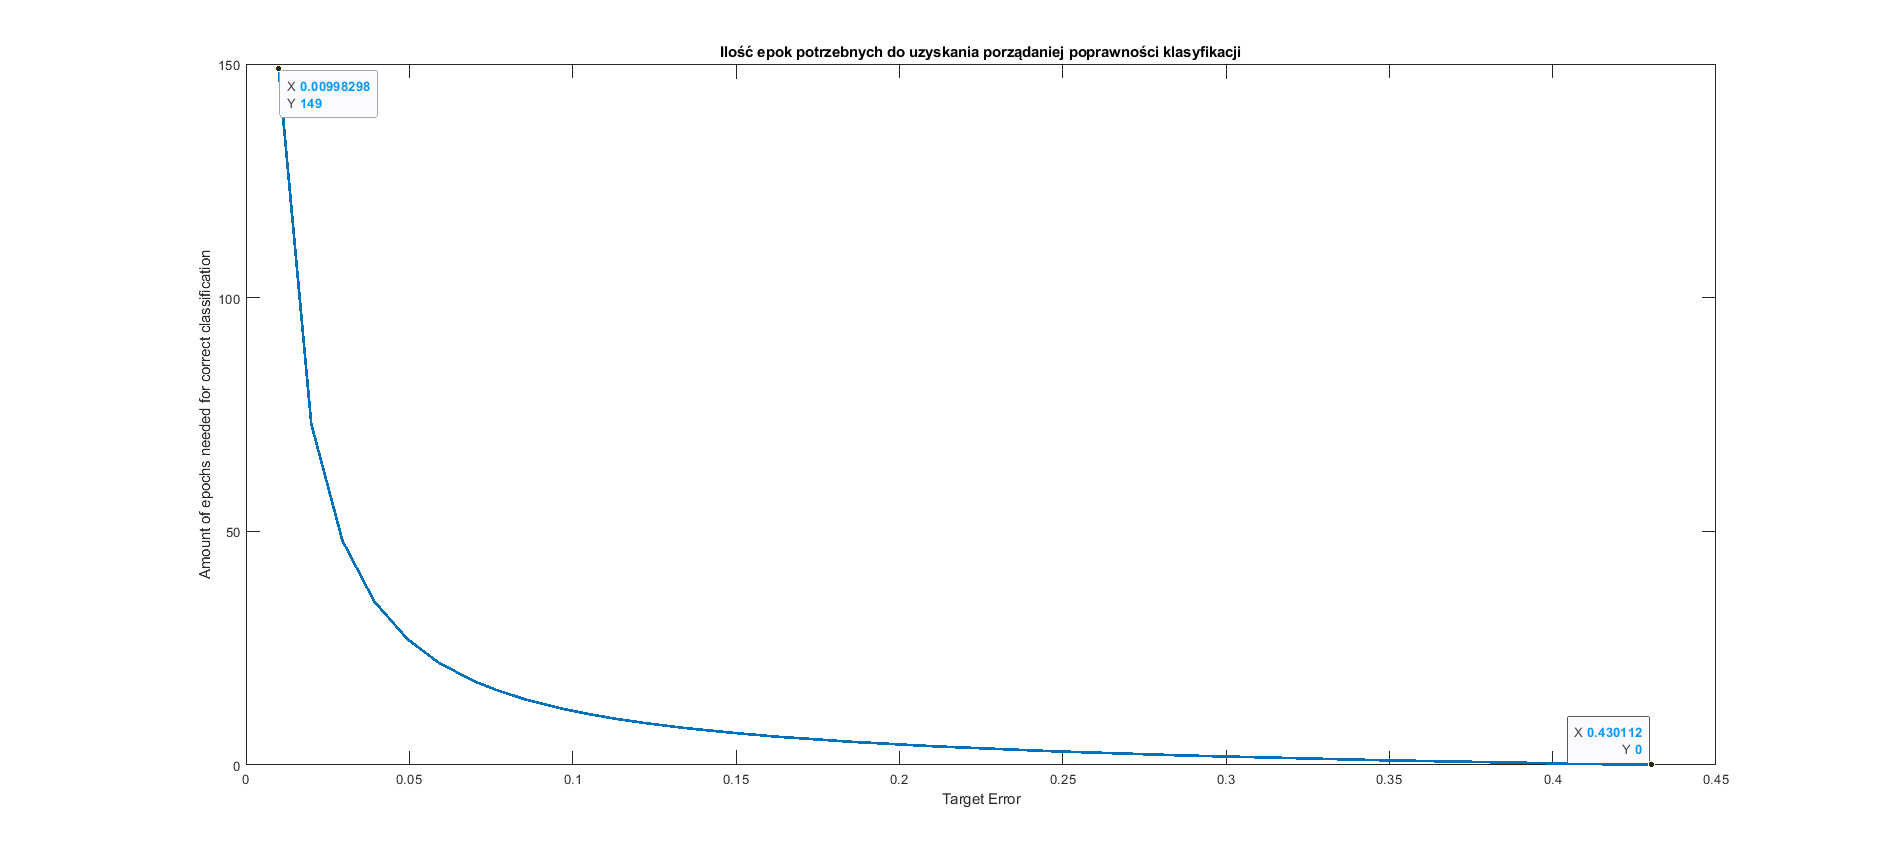
\includegraphics[width=15cm]{figures/target_epo_eta=0_1.png}
	\caption{Wykres do eksperymentu czwartego}
\end{figure}
Tutaj został powtórzony eksperyment trzeci lecz ze zmienionym learning rate na wartość 0,1 w przeciwieństwu to poprzedniego 0,01.
\newpage

\subsection{Eksperyment 5}
Celem piątego eksperymentu było sprawdzenie jak ilość neuronów w pierwszej wartstwie wpływa na szybkość uczenia się sieci.
W tym eksperymencie parametry sieci dwuwarstwowej były następujące:
\begin{itemize}
	\item epoki - 10000
	\item learning rate - 0,1
	\item batch size - 1
	\item target error - 0,18
\end{itemize}
\begin{figure}[ht!]
	\centering
	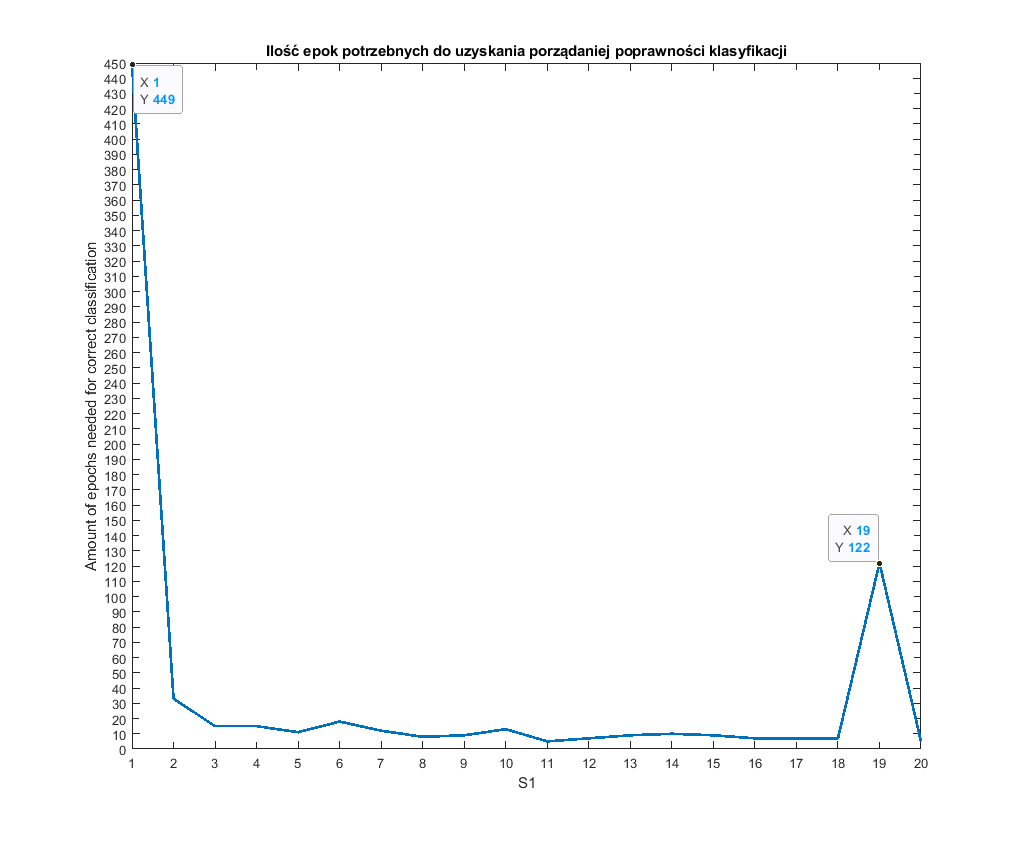
\includegraphics[width=15cm]{figures/S1_epo.png}
	\caption{Wykres do eksperymentu piątego}
\end{figure}
Na wykresie możemy zauważyć ewidenty spadek ilości epok potrzebnych do osiągniecia porządanej klasyfikacji wraz ze wzrostem ilości neuronów w warstwie S1, za wyjątkiem jednego wzrostu w przypadku 19 neuronów.
\newpage

\subsection{Eksperyment 6}
Celem szóstego eksperymentu było sprawdzenie jak ilość neuronów w drugiej wartstwie wpływa na szybkość uczenia się sieci.
W tym eksperymencie parametry sieci trójwarstwowej były następujące:
\begin{itemize}
	\item epoki - 10000
	\item learning rate - 0,1
	\item batch size - 1
	\item target error - 0,18
	\item S1 - 1
\end{itemize}
\begin{figure}[ht!]
	\centering
	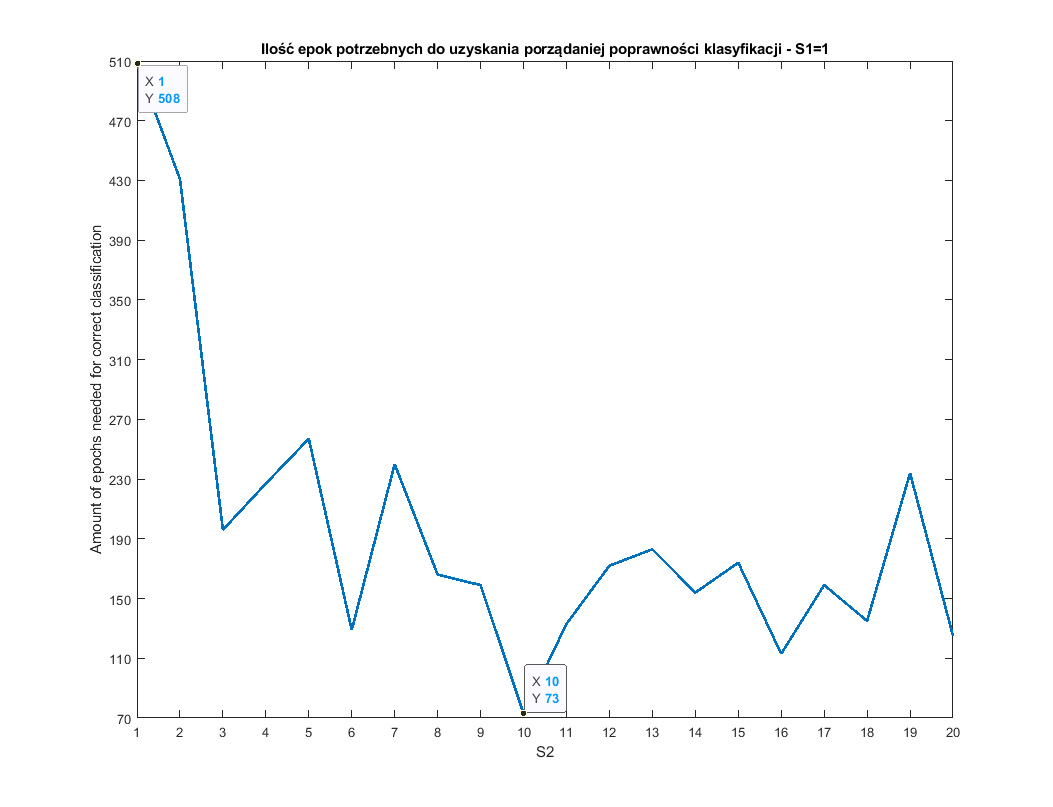
\includegraphics[width=14cm]{figures/S1=1_S2_epo.png}
	\caption{Wykres do eksperymentu szóstego}
\end{figure}
Pierwszy eksperyment zawierający sieć trójwarstwową, w tym eksperymencie chciałem sprawdzić jak sieć radzi sobie z nieoptymalną ilością neuronów w warstwie S1 (tylko jeden neuron), ilość neuronów w warstwie S2 jest natomiast zmienna w zakresie od 1 do 20.
\newpage

\subsection{Eksperyment 7}
Celem siódmego eksperymentu było sprawdzenie jak ilość neuronów w drugiej wartstwie wpływa na szybkość uczenia się sieci.
W tym eksperymencie parametry sieci trójwarstwowej były następujące:
\begin{itemize}
	\item epoki - 10000
	\item learning rate - 0,1
	\item batch size - 1
	\item target error - 0,18
	\item S1 - 2
\end{itemize}
\begin{figure}[ht!]
	\centering
	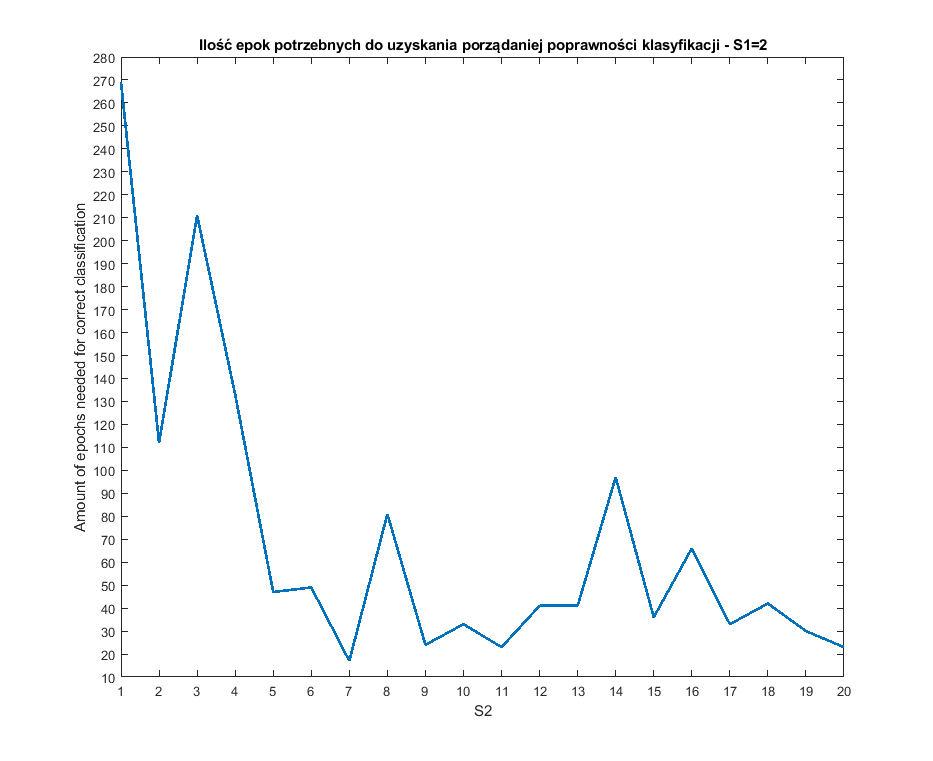
\includegraphics[width=15cm]{figures/S1=2_S2_epo.png}
	\caption{Wykres do eksperymentu siódmego}
\end{figure}
Tutaj został powtórzony eksperyment siódmy lecz ilość neuronów w warstwie S1 wynosiła 2, co znacznie poprawiło szybkość uczenia się sieci.
\newpage

\subsection{Eksperyment 8}
Celem ósmego eksperymentu było sprawdzenie jak ilość neuronów w pierwszej i drugiej wartstwie wpływa na szybkość uczenia się sieci.
W tym eksperymencie parametry sieci trójwarstwowej były następujące:
\begin{itemize}
	\item epoki - 10000
	\item learning rate - 0,1
	\item batch size - 1
	\item target error - 0,18
\end{itemize}
\begin{figure}[ht!]
	\centering
	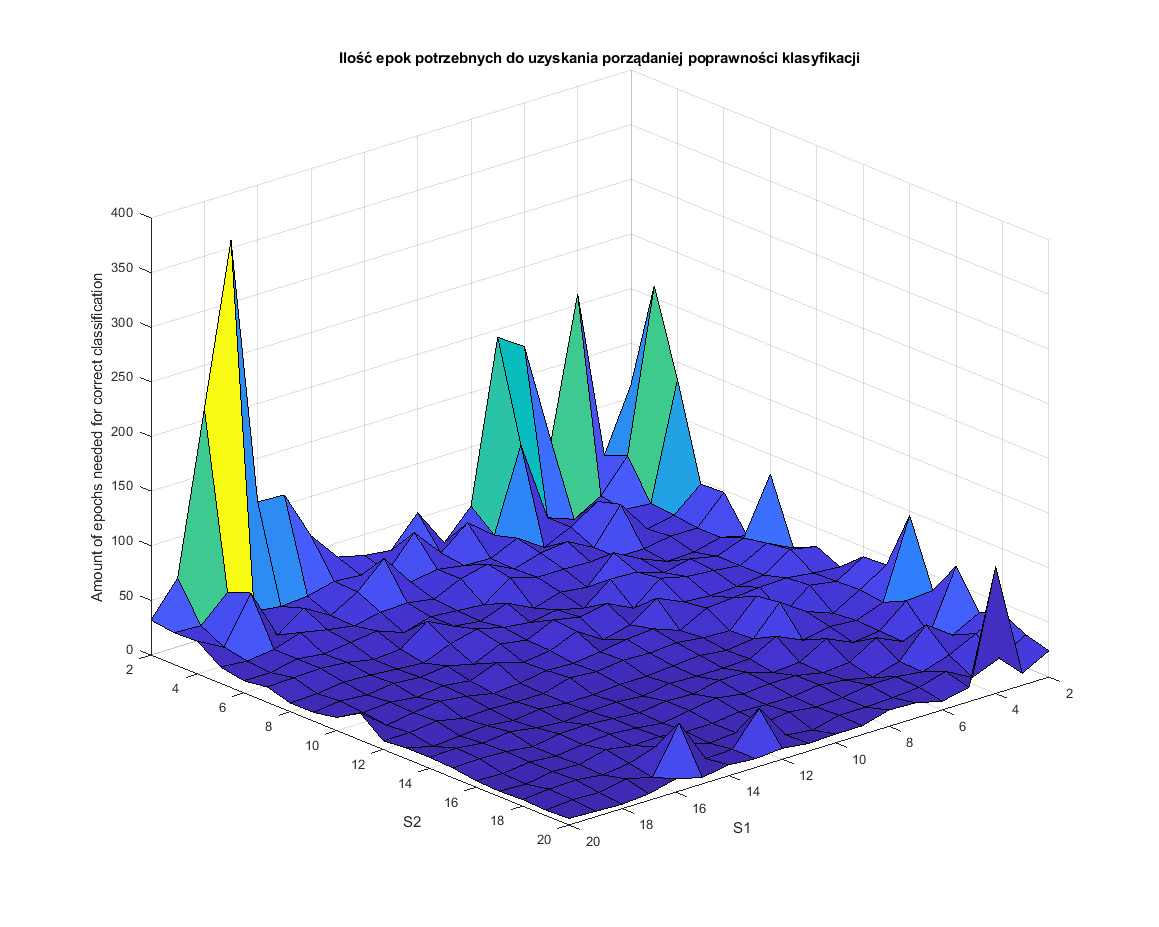
\includegraphics[width=15cm]{figures/S1=2+_S2=2+_epo.png}
	\caption{Wykres do eksperymentu ósmego}
\end{figure}
W tym eksperymencie sprawdzam jak zmienna ilość neuronów w warstwie S1 i S2 w zakresie od 2 do 20 neuronów wpływa na szybkość uczenia się sieci. Możemy zauważyć, że już w przypadku 8 neuronów w obydwu warstwach sieć uczy się już bardzo szybko.
\newpage


\clearpage

\section{Wnioski}

Celem projektu było zrealizowanie szutucznej sieci neuronowej uczonej algorytmem wstecznej propagacji błędu. W tym czelu użyto własnej implementacji sieci neuronowej napisanej w języku programowania Python na podstawie książki Michaela Nielsena.

Zbiór danych przeze mnie wykorzystywany okazał się być zbiorem liniowo separowalnym co wpłynęło na bardzo szybkie uczenie się sieci oraz pozwoliło na osiągnięcie 100\% poprawności klasyfikacji.

Przeprowadzone przeze mnie eksperymenty pozwoliły określić najoptymalniejsze parametry sieci neuronowej pozwalające nauczyć sieć w jak najktrótrszym czasie zachowując przy tym jak największą dokładność. Porównując różną ilość warstw oraz neuronów sieci dla mojego zestawu danych zauważyłem, że szybkość uczenia się sieci nie wzrastała wraz ze wzrostem ilości warstw oraz neuronów. Finalnie stwierdzono, że najoptymalniejszą konfigurajcą sieci będzie sieć jednowarstwowa z następującymi parametrami:
\begin{itemize}
	\item Ilość neuronów w warstwie wyjściowej = 2
	\item ETA (learning rate) = 0,1
	\item Batch size = 1
	\item Target error = 0,18
\end{itemize}
Konfiguracja ta wynika z tego, iż zestaw danych uczących jest jak zostało wspomniane wcześniej liniowo separowalny.

Podsumowując, zbiór danych oraz dobrane do niego parametry mają bardzo duży wpływ na dokładność oraz szybkość uczenia się sieci neuronowych. Niemożliwe jest określenie uniwersalnych parametrów, które działałyby jednakowo dobrze dla wszystkich możliwych zestawów danych oraz każdego typu sieci neuronowej.

Jednakowoż można stwierdzić, że do każdego zestawu danych można dobrać najoptymalniejszy rodzaj sieci i parametrów uczących pozwalających na najdokładniejsze i najszybsze rozwiązanie problemu. 
\clearpage

\addcontentsline{toc}{section}{Literatura}

\begin{thebibliography}{4}
\bibitem{dataset} https://archive.ics.uci.edu/ml/datasets/Acute+Inflammations
\bibitem{nielsen} Michael Nielsen, Neural Networks and Deep Learning.
\bibitem{zajdel1} Zajdel.R „Ćwiczenie 6 Model Neuronu”, Rzeszów, KIiA, PRz
\bibitem{zajdel2} Zajdel.R „Ćwiczenie 8 Sieć jednokierunkowa jednowarstwowa”, Rzeszów,KIiA,PRz
\bibitem{zajdel3} Zajdel.R „Ćwiczenie 9 Sieć jednokierunkowa wielowarstwowa”, Rzeszów,KIiA,PRz
\bibitem{tadusie} R.Tadeusiewicz, M.Szaleniec „Leksykon sieci neuronowych”
\end{thebibliography}

\clearpage

\end{document} 